%
% exemplo genérico de uso da classe iiufrgs.cls
% $Id: iiufrgs.tex,v 1.1.1.1 2005/01/18 23:54:42 avila Exp $
%
% This is an example file and is hereby explicitly put in the
% public domain.
%
\documentclass[cic,dipl,english]{iiufrgs} % pode-se usar 'dipl' em vez de 'tc'
% um tipo específico de monografia pode ser informado como parâmetro opcional:
%\documentclass[tese]{iiufrgs}
% monografias em inglês devem receber o parâmetro `english':
%\documentclass[diss,english]{iiufrgs}
% a opção `openright' pode ser usada para forçar inícios de capítulos
% em páginas ímpares
% \documentclass[openright]{iiufrgs}
% para gerar uma versão somente-frente, basta utilizar a opção `oneside':
% \documentclass[oneside]{iiufrgs}
\usepackage[T1]{fontenc}        % pacote para conj. de caracteres correto
\usepackage[utf8]{inputenc}   % pacote para acentuação
\usepackage{graphicx}           % pacote para importar figuras
%\usepackage[outdir=./]{epstopdf}
%\usepackage{epstopdf} 
\usepackage{times}              % pacote para usar fonte Adobe Times
%\usepackage{mathptmx}          % p/ usar fonte Adobe Times nas fórmulas

%
% Informações gerais
%
\title{Towards a Software Metric for OSGi}

\author{Mauricio Pestano}{Rafael}
% alguns documentos podem ter varios autores:
%\author{Flaumann}{Frida Gutenberg}
%\author{Flaumann}{Klaus Gutenberg}

% orientador e co-orientador são opcionais (não diga isso pra eles :))
\advisor[Prof.~Dr.]{Fernando Resin Geyer}{Cláudio}
\coadvisor[Prof.~Dr.]{DONSEZ}{Didier}

% a data deve ser a da defesa; se nao especificada, são gerados
% mes e ano correntes
%\date{maio}{2001}

% o nome do curso pode ser redefinido (ex. para TCs)
\course{Bachelor of Computer Science}
\def\ufrgs{Federal University of Rio Grande do Sul}
\def\ii{Informatics Institute}
\renewcommand{\titlepagespecificinfo}{Graduation Thesis}


% o local de realização do trabalho pode ser especificado (ex. para TCs)
% com o comando \location:
%\location{Itaquaquecetuba}{SP}

% itens individuais da nominata podem ser redefinidos com os comandos
% abaixo:
\renewcommand{\nominataCoordCICname}{Coordenador do Curso de CIC}
% \renewcommand{\nominataPRE}{Prof.~Jos{\'e} Carlos Ferraz Hennemann}
% \renewcommand{\nominataPREname}{Pr{\'o}-Reitor de Ensino}
% \renewcommand{\nominataPRAPG}{Prof\textsuperscript{a}.~Joc{\'e}lia Grazia}
% \renewcommand{\nominataPRAPGname}{Pr{\'o}-Reitora Adjunta de P{\'o}s-Gradua{\c{c}}{\~a}o}
% \renewcommand{\nominataDir}{Prof.~Philippe Olivier Alexandre Navaux}
% \renewcommand{\nominataDirname}{Diretor do Instituto de Inform{\'a}tica}
% \renewcommand{\nominataCoord}{Prof.~Carlos Alberto Heuser}
% \renewcommand{\nominataCoordname}{Coordenador do PPGC}
% \renewcommand{\nominataBibchefe}{Beatriz Regina Bastos Haro}
% \renewcommand{\nominataBibchefename}{Bibliotec{\'a}ria-chefe do Instituto de Inform{\'a}tica}
% \renewcommand{\nominataChefeINA}{Prof.~Jos{\'e} Valdeni de Lima}
% \renewcommand{\nominataChefeINAname}{Chefe do \deptINA}
% \renewcommand{\nominataChefeINT}{Prof.~Leila Ribeiro}
% \renewcommand{\nominataChefeINTname}{Chefe do \deptINT}

% A seguir são apresentados comandos específicos para alguns
% tipos de documentos.

% Relatório de Pesquisa [rp]:
% \rp{123}             % numero do rp
% \financ{CNPq, CAPES} % orgaos financiadores

% Trabalho Individual [ti]:
% \ti{123}     % numero do TI
% \ti[II]{456} % no caso de ser o segundo TI

% Trabalho de Conclusão [tc]:
% além de definir explicitamente o nome do curso (\course) e o local
% de realização (\location), é necessário redefinir a nominata,
% pois as informações necessárias dependem do curso. Ex.:
%\renewcommand{\nominata}{
%        FEDERAL UNIVERSITY OF RIO GRANDE DO SUL\\
%        Reitora: Prof\textsuperscript{a}.~Wrana Maria Panizzi\\
%        Pró-Reitor de Ensino: Prof.~José Carlos Ferraz Hennemann\\
%        Diretor do Instituto de Informática: Prof.~Philippe Olivier Alexandre Navaux\\
%        Coordenador do curso: Prof.~Seu Creysson\\
%        Bibliotecária-chefe do Instituto de Informática: Beatriz Regina Bastos Haro
%}

% Monografias de Especialização [espec]:
% \espec{Redes e Sistemas Distribuídos}      % nome do curso
% \coord[Profa.~Dra.]{Weber}{Taisy da Silva} % coordenador do curso
% \dept{INA}                                 % departamento relacionado

%
% palavras-chave
% iniciar todas com letras minúsculas, exceto no caso de abreviaturas
%
\keyword{OSGi}
\keyword{java}
\keyword{quality}
\keyword{metrics}
\keyword{modularity}


%
% inicio do documento
%
\begin{document}

% folha de rosto
% às vezes é necessário redefinir algum comando logo antes de produzir
% a folha de rosto:
% \renewcommand{\coordname}{Coordenadora do Curso}
\maketitle

% dedicatoria
\clearpage
\begin{flushright}
\mbox{}\vfill
{\sffamily\itshape
``If I have seen farther than others,\\
it is because I stood on the shoulders of giants.''\\}
--- \textsc{Sir~Isaac Newton}
\end{flushright}


% agradecimentos
\chapter*{Agradecimentos}
Agradeçimentos


% sumario
\tableofcontents

% lista de figuras
\listoffigures

% lista de tabelas
%\listoftables

% lista de abreviaturas e siglas
% o parametro deve ser a abreviatura mais longa
\begin{listofabbrv}{SPMD}
        \item[SMP] Symmetric Multi-Processor
        \item[NUMA] Non-Uniform Memory Access
        \item[SIMD] Single Instruction Multiple Data
        \item[SPMD] Single Program Multiple Data
        \item[ABNT] Associação Brasileira de Normas Técnicas
\end{listofabbrv}


% idem para a lista de símbolos
%\begin{listofsymbols}{$\alpha\beta\pi\omega$}
%       \item[$\sum{\frac{a}{b}}$] Somatório do produtório
%       \item[$\alpha\beta\pi\omega$] Fator de inconstância do resultado
%\end{listofsymbols}

% aqui comeca o texto propriamente dito

\begin{abstract}{}{OSGi, Java, quality metrics, modularity}
 Todays software applications are becoming more complex, bigger, dynamic and harder to maintain. One way to overcome nowadays complexities is to build modular applications so we can divide the problems into small blocks which collaborate to solve bigger problems, the so called \emph{divide to conquer}. Another important aspect in the software industry that helps building large applications is the notion of software quality because its well known that higher quality softwares are easier to maintain and evolve at long term.

The Open Services Gateway Initiative(OSGi) is the \emph{de facto} standard for building Java modular applications but there is no automated way to measure the quality of an OSGi system. In the context of Java applications there are many well known quality metrics to measure application's quality but when we move to Java modular applications where standard quality metrics does not fit or even exist we run out of options. 

In this work we will present a tool for analyzing OSGi applications and measure their quality. We also propose 6 metrics based on good practices inside OSGi world and apply them on top of 10 real OSGi projects which vary in size, teams and domain of solution. 
\end{abstract}



\begin{englishabstract}{}{OSGi, java, quality, metrics, modularity}
As aplicações de software hoje em dia estão cada vez mais complexas, maiores, dinâmicas e mais difíceis de manter. Uma maneira de superar as complexidades dos sistemas modernos é através de aplicações modulares as quais são dividas em partes manores que colaboram entre si para resolver problemas maiores, o famoso \emph{dividir para conquistar}. Outro aspecto importante na industria de software que ajuda à construir aplicações grandes é o conceito de qualidade de software já que é sabido que quanto maior a qualidade do software mais facil de mante-lo e evolui-lo a logo prazo será.

The Open Services Gateway Initiative(OSGi) é o \emph{padrão de fato} para se criar aplicações modulares em java porém não existe forma automatizada de se medir a qualidade de sistemas OSGi. No ambito de aplicações java existem diversas metricas de qualidade e ferramentas para medir a qualidade de softwar mas quando entramos no contexto de aplicações modulares, onde as métricas conhecidas não se encaixam ou não existem, ficamos sem opções. 

Neste trabalho será apresentada uma ferramenta chamada \emph{Intrabundle} que analisa projetos OSGi a mede sua qualidade. Ainda seram propostas métricas de qualidade baseadas em boas práticas conhecidas do mundo OSGi que serão aplicadas em 10 projetos reais que variam em tamanho, equipes e domínio.
\end{englishabstract}


%introdução
% introducao
\chapter{Introduction}
 This chapter will drive the reader through the context and motivation of this work followed by the objectives and later the organization of this text is presented.  
 

\section{Context}

% stating how important quality is % 
One of the pillars of sustainable software development is its quality which can basically be defined as internal and external where the first focuses on how software meets its specification and works accordingly to its requirements and the second is aimed on how well the software is structured and designed. To measure external quality there is the need to execute the software\footnote{Also known as dynamic analysis} either by an end user accessing the system or an automated process like for example functional testing or performance testing. Internal quality however can be verified by either \emph{statical analysis} that is mainly the inspection of the source code itself or by dynamic analysis which means executing the software like for example automated \emph{whitebox testing}, the detailed investigation of internal logic and structure of the code \citep{Khan 2012}.   

With good software quality in mind we take applications to another level where maintainability is increased, correctness is enhanced, defects are identified in early development stages, which can lead up to 100 times reduced costs \citep{Beohm 2001}, and also other characteristics like reusability, reliability and portability are benefited by higher software quality.  

% OSGi and its importance %
A well known and successful way to structure software architecture is to modularize its components. In the Java ecosystem although there is a moving to modularize the JDK and Java applications with the project Jigsaw \citep{Krill 2012} and also the recent \emph{microservices} movement \citep{Knorr 2014}. Today the only practical working and well known solution for modular Java applications is OSGi, a very popular component-based and service-oriented framework for building Java modular applications which is the \emph{de facto} standard solution for this kind of software since early 2000's and have being used as basis of most JavaEE application servers, the open source IDE Eclipse, Atlassian Jira and Confluence to cite a few big players using OSGi. 

In the context of Java modular applications using OSGi and software quality there is no known standard way neither tools to measure OSGi projects \textit{internal quality} \citep{Hamza 2013} although for \emph{external quality} the classical approaches like automated testing are sufficient and widely used.

        
\section{Objectives}
The main objective of this work is to create software metrics to measure internal quality of OSGi based projects where this metrics must reflect good practices in the OSGi world.

Another aim of this work is to create a tool to apply and validate the metrics on real OSGi projects and finally analyze the resulting qualities produced by the tool.  

 
\section{Organization}

This text is organized in the following way. First chapter defines the context, motivation and objectives of this work. The second chapter will introduce the main concepts and technologies used in this work and will be divided into two main sections where the first will be focused in the area of software quality like quality measurement, quality metrics, program analysis and quality analysis tools and the second section of chapter two will present Java and OSGi, how standard Java and OSGi are different in respect to quality metrics and why we need different metrics for OSGi. The third chapter presents \textbf{Intrabundle}, an OSGi code introspection tool to measure internal quality, we will see how Intrabundle works, what kind of information it extracts and what metrics it is applying. The fourth chapter will analyze the results Intrabundle produces and validate them to decide if this work has a valid contribution or not. The last chapter will present the conclusions and future work on this subject.
% e aqui vai a parte principal
 
% \chapter{Estado da arte}
\chapter{State of Art}
This chapter presents an overview of the concepts and technologies that were studied and used on the development of this work. 
In section \textit{2.1 - Software Quality}, will be presented general aspects of software quality such as \textit{quality measurement},  \textit{software metrics}, \textit{program analysis} and some tools that are used in this area.  

Section \textit{2.2 - Java and OSGi} will introduce OSGi a framework for build service oriented Java modular applications as well the motivation 
behind this solution and why standard quality metrics aren't sufficient for this kind of application. 


\section{Software Quality}

There has been many definitions of software quality(TODO REF - Metrics and Models in Software Quality Engineering) and there is even an ISO norm for it, the ISO/IEC 25010 \citep{iso 2011}. All this definitions agree that the main motivation to perform continuous software quality management is to avoid \textbf{software failures} and increase \textbf{maintainability} in the sense that the more quality a program has the easier will be to maintain, the less bugs or abnormal behavior it will have and the more it will conform with its functional and non functional requirements\footnote{Functional and non functional requirements can be simply defined as \textit{what} the software does and \textit{how} the software will do respectively}. 

Another important aspect of software quality is that it can be divided in two groups, the \textbf{external} and \textbf{internal} quality. When we talk about \textit{external quality} we are aiming to the user view which is the one that sees the software working and use it, this kind of quality is usually enforced through software testing. External quality can also be mapped to functional requirements so the greater external quality is the more usable and less defects it will have for example. The opposite is internal or structural quality that aims to how the software is architect-ed internally which is the perspective of the programmer and non functional requirements so the higher internal quality the better the code is structured, efficient, robust and maintainable it should be. Image 2.1 illustrates internal and external quality and its target audience.


\begin{figure}[h]
\caption{Internal and external quality audience}
\centering
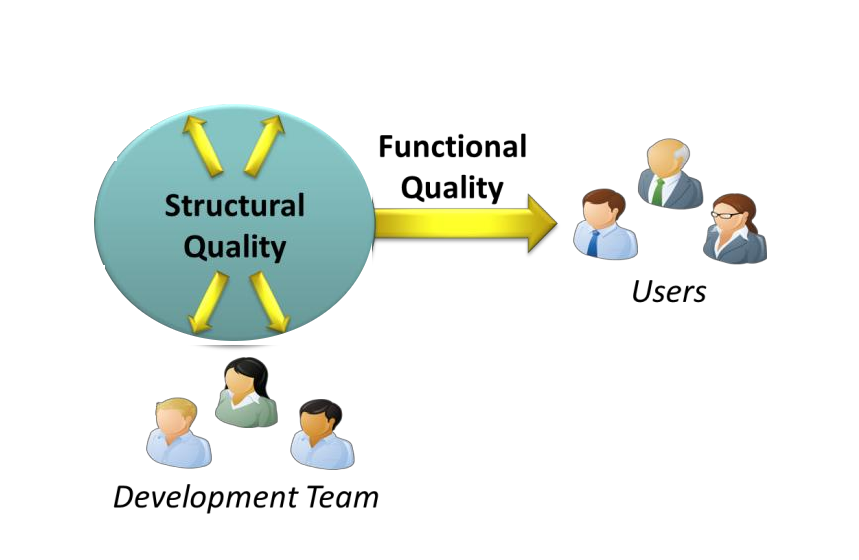
\includegraphics[scale=0.5]{external-internal-quality}
\end{figure}
\FloatBarrier

% functional quality(performed via automated testing)
% structural quality(\textbf{this is where our work shines})

\subsection{Quality Measurement}
Quality measurement focuses on quantifying software desirable characteristics and each characteristic can have a set of measurable attributes, for example \textit{high cohesion} is a desirable characteristic and \textit{LOC - lines of code} is a measurable attribute related to cohesion. Quality measurement is close related to internal quality and in most cases is performed via static code analysis where program code is inspected to search for quality attributes to be measured but in some cases a dynamic analysis, where the program analysis is done during software execution, can be performed to measure characteristics that can be perceived only when software is running, for example performance or code coverage\footnote{A technique that measures the code lines that are executed for a given set of software tests, its also considered a software metric.}.     

In the extent of this work the characteristics of software to be considered and measured later are listed and described in table 2.1:  

\begin{table}[h]
\caption{Quality characteristics to be considered}
\begin{center}
    \begin{tabular}{  p{3cm} | p{8cm} | p{5cm} }
    \hline
    Characteristic & Description & OSGi example \\  \hline
    Reliability & the degree to which a system or component performs its required functions under stated conditions for a specified period of time. & Bundles should not have stale service references.\\ \hline
    Performance Efficiency & Performance relative to the amount of resources used under stated conditions for a specified
period of time. & Bundle startup time, also bundle dependency can decrease performance. \\ \hline
    Security & the degree of protection of information and data so that unauthorized persons or systems cannot read, access or modify them. & Bundles should declare permissions \\ \hline
    Maintainability & The degree to which the product can be modified. & Modules should be loosely coupled, bundles should publish only interfaces etc. \\ 
    \hline
     
    \end{tabular}
    Source: \cite{cisq 2012}
\end{center}
\end{table}
\FloatBarrier

\subsection{Software Metric}
A software metric is the measurement of a software attribute which in turn is a quantitative calculation of a characteristic.
\subsubsection{Common Software Metrics}
The table 2.2 below shows some well known software metrics and its description:

\begin{table}[h]
\caption{Common Software metrics}
\begin{center}
    \begin{tabular}{  p{3cm} | p{8cm} }
    \hline
    Metric & Description \\  \hline
    Cyclomatic complexity & It is a quantitative measure of the complexity of programming instructions.\\ \hline
    Cohesion & measure the dependency between units of code like for example classes in object oriented programing or modules in modular programming like OSGi. \\ \hline
    Coupling & measures how well two software components are data related or how dependent they are. \\ \hline
    Lines of code (LOC) & used to measure the size of a computer program by counting the number of lines in the text of the program's source code. \\ \hline
    Code coverage & measures the code lines that are executed for a given set of software tests \\ \hline
    Function point analysis (FPA) & used to measure the size (functions) of software. \\
    \hline

    \end{tabular}
    \\*Source: \cite{sqa 2012}
\end{center}
\end{table}

\FloatBarrier

\subsection{Program Analysis}
Program analysis sis the process of automatically analyzing the behavior of computer programs. Two main approaches in program analysis are \textbf{static program analysis} and \textbf{dynamic program analysis}. Main applications of program analysis are program correctness, program optimization and quality measurement.

\subsubsection{Static Program Analysis}
 Is the analysis of computer software that is performed without actually executing programs \citep{Wichmann 1995}. In this kind of analysis source code is inspected and valuable information is collected based on its internal structure and components. 

\subsubsection{Dynamic Program Analysis}
Is a technique that analyze the system's behavior on the fly, while it is executing. The main objectives of this kind of analyze is to catch \textit{memory leaks}\footnote{Resources that are hold on system's memory and aren't released}, identify arithmetic errors and extract code coverage. 


\subsection{Quality Analysis Tools}

The table 2.3 lists some code quality analysis tools in the Java ecosystem:

\begin{table}[h]
\caption{Quality analysis tools}
\begin{center}
    \begin{tabular}{  p{3cm} | p{8cm} | p{2cm} }
    \hline
    Name & Description & Type\\  \hline
    \href{http://www.sonarqube.org}{SonarQube} &  An open source platform for continuous inspection of code quality. & static\\ \hline
    \href{http://findbugs.sourceforge.net/}{FindBugs} & An open-source static bytecode analyzer for Java. & static\\ \hline 
    \href{http://checkstyle.sourceforge.net/}{Checkstyle} & A static code analysis tool used in software development for checking if Java source code complies with coding rules. & static\\ \hline 
    \href{pmd.sourceforge.net/}{PMD} & A static ruleset based Java source code analyzer that identifies potential problems. & static\\ \hline 
    \href{http://www.contemplateltd.com/threadsafe}{ThreadSafe} & A static analysis tool for Java focused on finding concurrency bugs. & static\\ \hline
    \href{http://www.intooitus.com/products/infusion}{InFusion} & Full control of architecture and design quality. & static\\ \hline 
    \href{https://www.ej-technologies.com/products/jprofiler/overview.html}{JProfiler} & helps you resolve performance bottlenecks, pin down memory leaks and understand threading issues & dynamic \\ \hline
    \href{http://www.eclemma.org/jacoco/}{JaCoCo} & A free code coverage library for Java. & dynamic\\ \hline 
    \href{https://code.google.com/p/javamelody/}{Javamelody} & Java or Java EE application Monitoring in QA and production environments. & dynamic\\ \hline 
    \href{http://www-304.ibm.com/partnerworld/gsd/solutiondetails.do?solution=23517&expand=true}{Introscope} & An application management solution that helps enterprises keep their mission-critical applications high-performing and available 24x7. & dynamic\\ \hline

    \end{tabular}
    %\\*Source: \cite{sqa 2012}
\end{center}
\end{table}

\FloatBarrier

Figure 2.2 shows the execution of static analysis on \textit{Intrabundle} using \textbf{PMD}, note that PMD is based on rules and Intrabundle break some of them(intentionally) like \textbf{Unused variables}, \textbf{EmptyCatchBlock} so PMD consider them compile failure and the project cannot be compiled until the rules are fixed in code:

\begin{figure}[h]
\caption{Intrabundle PMD rule violation}
\centering
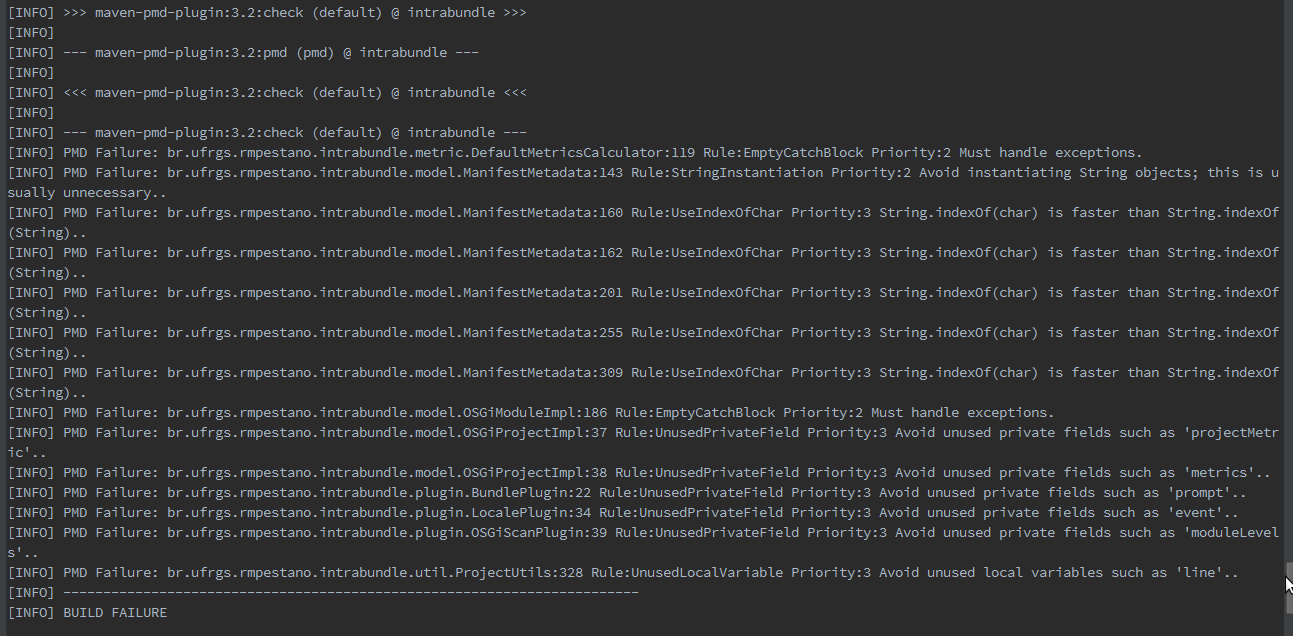
\includegraphics[scale=0.5]{intrabundle-pmd-build-failure}
\end{figure}

\FloatBarrier

The rules are totally customizable via xml configuration, Intrabundle PMD rules are shown in figure 2.3:

\begin{figure}[h]
\caption{Intrabunde PMD ruleset}
\centering
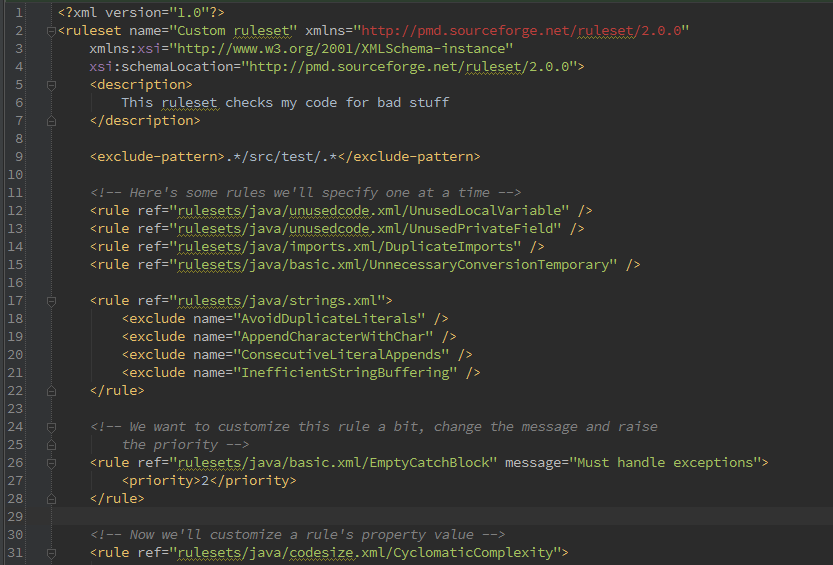
\includegraphics[scale=0.5]{intrabundle-pmd-ruleset}
\\*Source: \cite{intrabundle pmd 2014}
\end{figure}

\FloatBarrier

\section{Java and OSGi}

In the context of Java™ programming language \citep{Arnold 2005}, which accordingly to IEEE spectrum of this year is the most popular programming language \citep{ieee spectrum 2014}, and modular applications this section will introduce the Java language and OSGi framework.

\subsection{The Java language}
Java is a general purpose object oriented\footnote{Object-oriented programming(OOP) integrates code and data using the concept of an "object" which is a piece of software that holds state and behavior} programming language created by Sun Microsystems in 1995 which aims on simplicity, readability and universality. Java runs on top of the so called JVM, the acronym for Java Virtual Machine, which is a abstract computing machine\footnote{Also known as \textit{Virtual Machine} which is an emulation of a particular computer system} and platform-independent execution environment that execute Java byte code\footnote{The intermediate output of the compilation of a program written in Java that can be read by the JVM} and converts it into host machine language(e.g. linux, windows etc...) allowing Java programs to "run everywhere" independently of operating system or platform. JVM implementations are different for each platform but the generated bytecode is the same, Figure 2.4 illustrates how JVM works:

\begin{figure}[h]
\caption{JVM architecture}
\centering
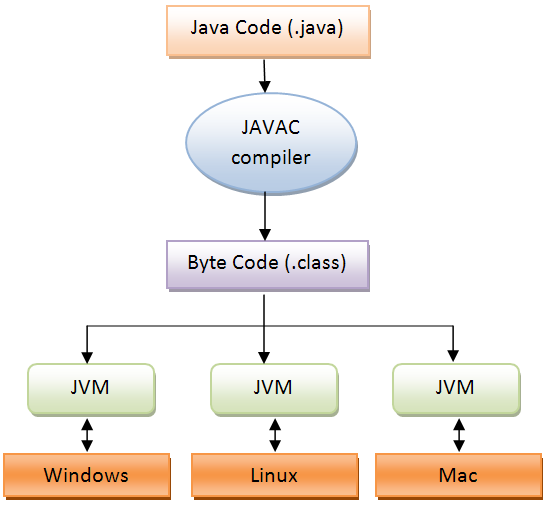
\includegraphics[scale=0.5]{jvm}
\end{figure}  
\FloatBarrier

Other aspects of Java are listed below:   

\begin{itemize}
\item Type safe\footnote{Type safety is the extent to which a programming language discourages or prevents type errors} 
\item Dynamic: during the execution of a program, Java can dynamically load classes 
\item Strong memory management(no explicit pointer)
\item Automatic garbage collection to release unused objects from memory
\item Robust: extensive compile-time checking so bugs can be found early
\item Multithreaded\footnote{Multithreading is a program’s capability to perform several tasks simultaneously}
\item Distributed: networking capability is inherently integrated into Java
\end{itemize}

\subsection{The OSGi framework}
% \chapter{Mais estado da arte}
\chapter{Mais estado da arte}
Capítulo para mais estado da arte


% \chapter{A minha contribuição}
\chapter{Intrabundle - An OSGi Bundle Introspection Tool}

\section{Introduction}

\section{Design Decisions}
To analyze large code bases of OSGi projects which can vary from KLOCs to thousands of KLOCs we needed a lightweight approach with the following functional requirements:

- 

The following alternatives were evaluated:

-

\section{JBoss Forge}

\section{Implementation Overview}

\section{Collecting Bundle Data}

\section{Metrics Calculation}

\section{Intrabundle Quality}
In this section we will see how intrabundle quality is managed and how some concepts of \textit{chapter 2 - State of art} were applied to the project.
\subsection{Internal quality}
Intrabundle internal is managed by PMD and JaCoCo. PMD is an static analysis tool and JaCoCo a dynamic analysis one. Both were presented at Chapter two in section \textit{Quality Analysis Tools} with the objective to guarantee non functional requirements.

\subsubsection{Example}
 A PMD was already illustrated at Chapter 2 as an example of static analysis tool. JaCoCo is used to calculate code coverage to track files and methods that automated tests are covering. Figure 3.1 shows JaCoCo code coverage report for Intrabundle:

\begin{figure}[h]
\caption{Intrabundle code coverage}
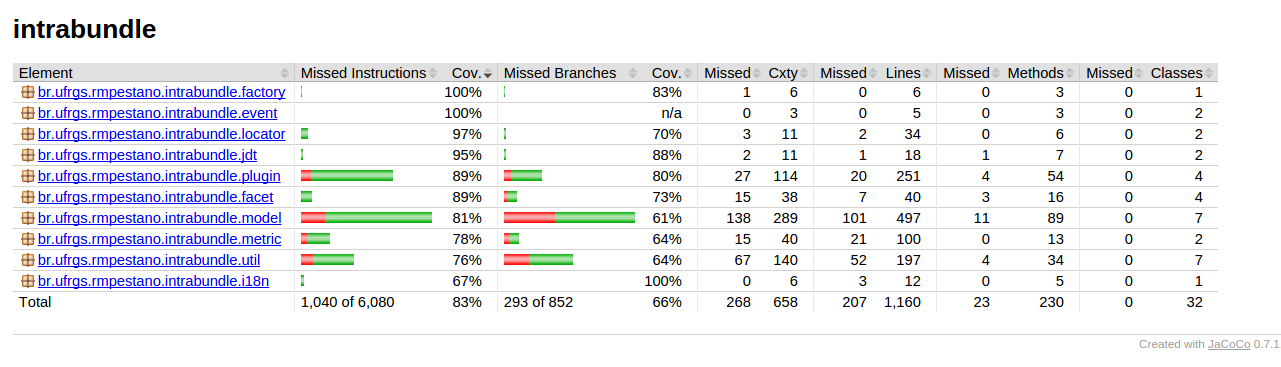
\includegraphics[scale=0.5]{intrabundle-code-coverage}
\end{figure}

\FloatBarrier

\subsection{External quality}
Intrabunde external quality is assured by automated whitebox tests so we can verify if Intrabundle is working as expected, if it meets its functional requirements.

\subsubsection{Example}
Intrabundle performs 62 \textbf{integration tests}, which can be defined as automated tests aimed to detect any inconsistencies between the software units that are integrated together, to guarantee its external quality. In this kind of automated tests the system must be running and in case of Intrabundle we also need the Forge runtime up and running during tests and that is done by Arquillian \citep{dan 2011}, an integration test platform. Figure 3.2 shows the result of integration tests execution:

\begin{figure}[h]
\caption{Intrabundle external tests}
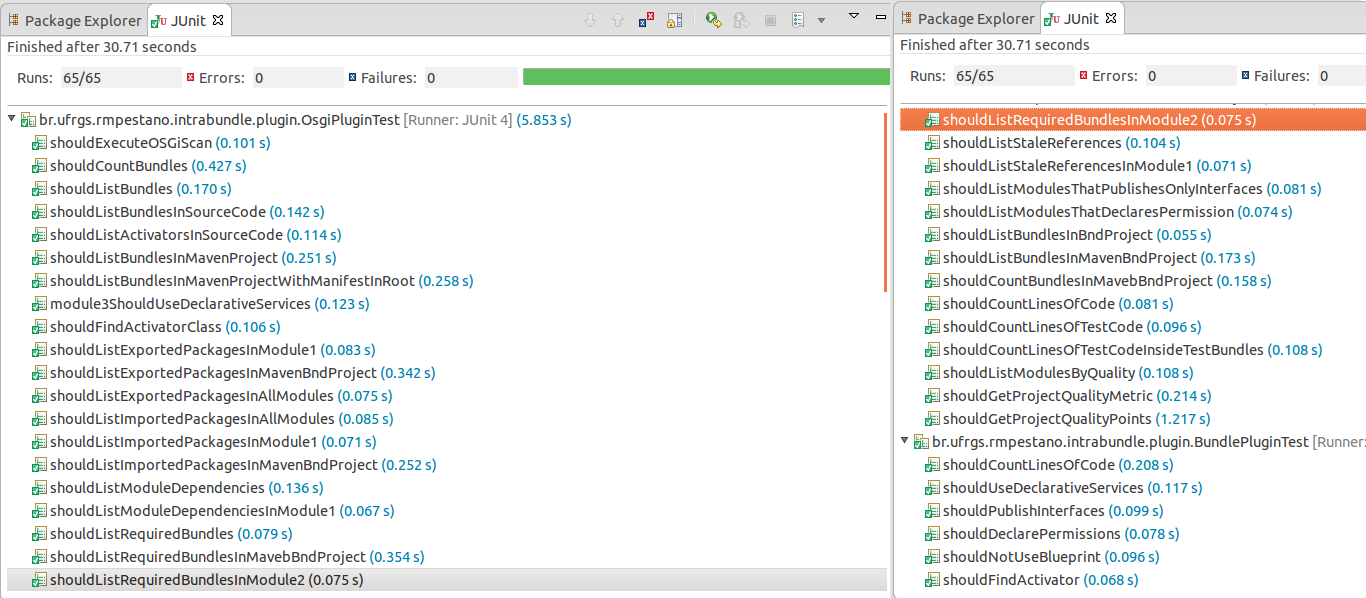
\includegraphics[scale=0.5]{intrabundle-external-quality}
\end{figure}

\FloatBarrier
% \chapter{Prova de que a minha contribuição é válida}
\chapter{Bundle Introspection Results}

This chapter will make a deep analysis of results and prove that my contribution is valid(or not)
% \chapter{Conclusão}
\chapter{Conclusão}
Capítulo para conclusão






% referencias
% aqui será usado o environment padrao `thebibliography'; porém, sugere-se
% seriamente o uso de BibTeX e do estilo abnt.bst (veja na página do
% UTUG)
%
% observe também o estilo meio estranho de alguns labels; isso é
% devido ao uso do pacote `natbib', que permite fazer citações de
% autores, ano, e diversas combinações desses
\begin{thebibliography}{este-parametro-nao-eh-usado-pelo-estilo-ABNT}

\bibitem[ANDREWS, 1991]{Andrews:CP-91} ANDREWS,
  G.~R\@. \textbf{Concurrent programming}: principles and
  practice. Redwood~City, USA: Benjamin/Cummings, 1991. 637p.
  
\bibitem[ASSENMACHER et~al.(1993)ASSENMACHER; BREITBACH; BUHLER;
  H{\"U}BSCH; SCHWARZ]{Assenmacher:Panda-ECOOP93} ASSENMACHER, H.;
  BREITBACH, T.; BUHLER, P.; H{\"U}BSCH, V.; SCHWARZ, R\@.
  Panda---supporting distributed programming in {C}++. In: EUROPEAN
  CONFERENCE ON OBJECT-ORIENTED PROGRAMMING, 7., 1993, Kaiserslautern,
  Germany. \textbf{Proceedings{\ldots}} Berlin: Springer-Verlag, 1993.
  p.361--383. (Lecture Notes in Computer Science, v.707).

\bibitem[BAKER; SMITH, 1996]{Baker:PP-96} BAKER, L.; SMITH,
  B.~J\@. \textbf{Parallel programming}. New~York: McGraw-Hill,
  1996. 381p.

\bibitem[CAROMEL; KLAUSER; VAYSSIERE, 1998]{Caromel:TSC-CPE-10-11-98}
  CAROMEL, D.; KLAUSER, W.; VAYSSIERE, J\@. Towards seamless computing
  and metacomputing in {J}ava.  \textbf{Concurrency: Practice and
  Experience}, West~Sussex, v.10, n.11--13, p.1043--1061,
  Sept./Nov.~1998.

\bibitem[FURMENTO; ROUDIER; SIEGEL, 1995]{Furmento:PDC-95} FURMENTO,
  N.; ROUDIER, Y.; SIEGEL, G\@. \textbf{Parall{\'e}lisme et
  distribution en {C}++}: une revue des langages existants. Valbonne,
  FR: I3S, Universit\'{e} de Nice Sophia-Antipolis, 1995. (RR~95-02).

\bibitem[INSTITUTE OF ELECTRICAL AND ELECTRONIC ENGINEERS,
  1995]{IEEE:Pthreads-95} INSTITUTE OF ELECTRICAL AND ELECTRONIC
  ENGINEERS\@. \textbf{Information Technology---Portable Operating
  System Interface (POSIX), Threads Extension [C Language]},
  \mbox{IEEE}~1003.1c-1995.  New~York, 1995.

\bibitem[SILBERSCHATZ; PETERSON; GALVIN, 1991]{Silberschatz:OSC-3-91}
  SILBERSCHATZ, A.; PETERSON, J.~L.; GALVIN, P.~B\@. \textbf{Operating
  system concepts}. 3.ed.  Reading, USA: Addison-Wesley, 1991. 696p.

\bibitem[UTUG(2001)UTUG]{UTUG:Homepage-01} UTUG\@. \textbf{Página do grupo
  de usuários {\TeX} da {UFRGS}}. Disponível em:
  $<$http://www.inf.ufrgs.br/utug$>$. Acesso em: maio 2001.

\bibitem[WILSON, 2001]{Wilson:MME-01} WILSON, P.~C\@. \textbf{Um
  método ótimo para o preparo de café em laboratório baseado na
  reciclagem de filtros}. 2001. 123p.  Disserta{\c{c}}{\~a}o (Mestrado
  em Ci{\^e}ncia da Computa{\c{c}}{\~a}o) --- Instituto de
  Inform{\'a}tica, Universidade Federal do Rio Grande do Sul,
  Porto~Alegre.

\end{thebibliography}

\end{document}
